%---------------------------------------------------------------------
\section{Ensemble Tests}
\label{sec:ensembles}

Several ensembles of pseudo-data events were produced from the
background model to test the performance of the analysis. These
ensembles include:
\vspace{-0.05in}
\begin{myenumerate}
\item 400 fake data samples with SM single top content
($\sigma_{tb+tqb}=2.86$~pb).
\item Four sets of 100 samples each (named A, B, C and D), with
unknown (to the analyzers) single top content, but with SM ratios
between the $tb$ and $tqb$ cross sections.
\item Two sets of 200 samples with the SM ratio between the $tb$ and
$tqb$ cross sections, and with a total single top cross section of
$\sigma_{tb+tqb}=4.5$~pb and $\sigma_{tb+tqb}=4.7$~pb.
% Uncomment once the final set of results and plots are done:
%\item 6 sets of 100 experiments with unknown total cross section and
%      unknown $tb$:$tqb$ ratio
\end{myenumerate}
\vspace{-0.05in}
The full analysis chain was run using each pseudo-dataset as if it
were the real dataset. The results are presented in the following
subsections.

\subsection{Ensemble Tests with SM Signal}
\label{ens_SM_sig}

Figure~\ref{SMens} shows the distribution of estimated cross sections
from one ensemble generated with the SM input signal cross sections
for the electron, muon, and e+$\mu$ channel. The ensemble contains 400
samples of both 2-jet and 3-jet events. The input cross section in
each case is 2.86~pb. The most probable value of the distribution is
2.75~pb while the mean is 3.18~pb.

\vspace{0.1in}
\begin{figure}[!h!tbp]
\includegraphics[width=0.40\textwidth]
{figures/ensembles/Ensembles_Electron}
\includegraphics[width=0.40\textwidth]
{figures/ensembles/Ensembles_Muon}
\includegraphics[width=0.40\textwidth]
{figures/ensembles/Ensembles}
\vspace{-0.1in}
\caption[SMens]{Results of standard model ensemble test for the
electron channel (upper left plot), the muon channel (upper right
plot), and electrons and muons combined (lower plot).}
\label{SMens}
\end{figure}

\clearpage

\subsection{Ensemble Tests with Non-SM Signal}
\label{ens_nonSM_sig}

Five more ensembles were generated with a non-SM $tb$+$tqb$ cross
section, but SM $tb$:$tqb$ cross section ratio ($\sigma_s/\sigma_t =
0.44$). The results are shown in Fig.~\ref{ensembles}.

\vspace{0.1in}
\begin{figure}[!h!tbp]
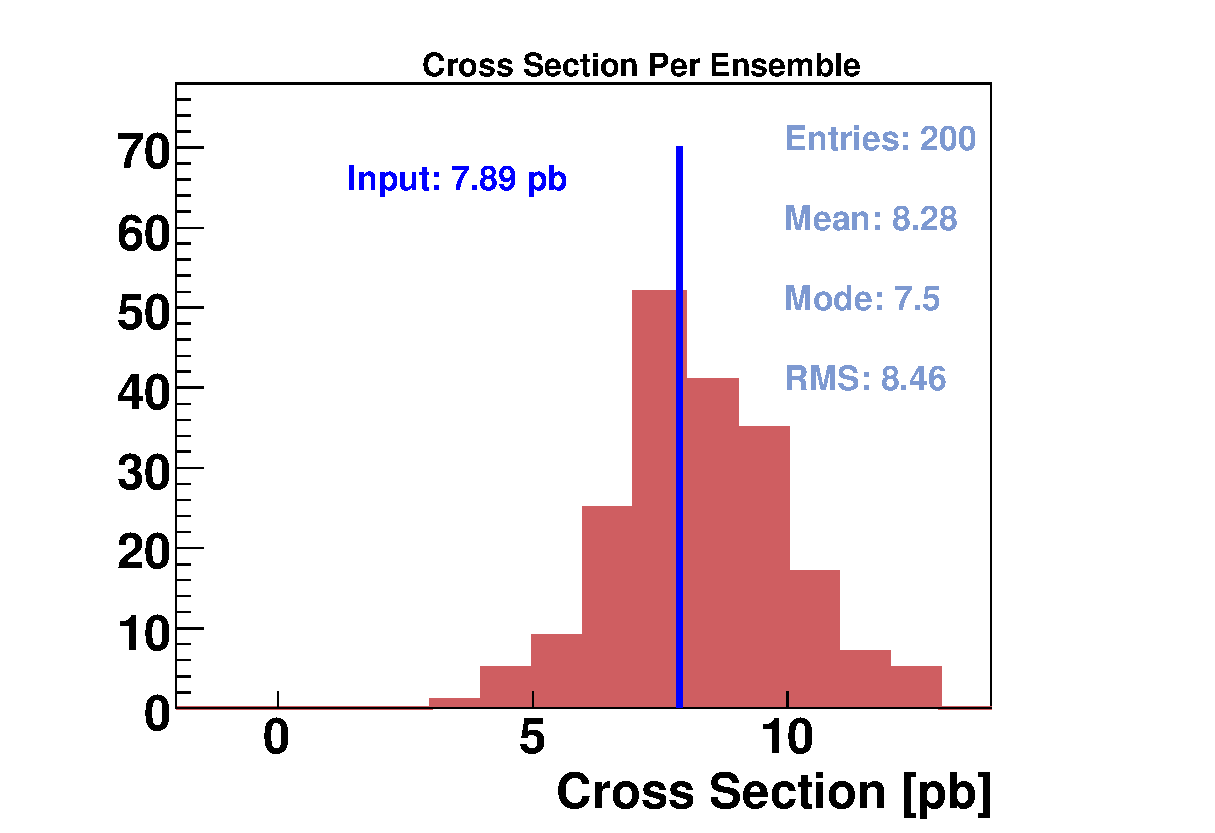
\includegraphics[width=0.40\textwidth]{figures/ensembles/EnsemblesA}
\includegraphics[width=0.40\textwidth]{figures/ensembles/Ensembles0sig1}
\includegraphics[width=0.40\textwidth]{figures/ensembles/EnsemblesC}
\includegraphics[width=0.40\textwidth]{figures/ensembles/EnsemblesD}
\includegraphics[width=0.40\textwidth]{figures/ensembles/Ensembles4.5.eps}
\includegraphics[width=0.40\textwidth]{figures/ensembles/Ensembles4.7.eps}
\vspace{-0.1in}
\caption{Results using the ensembles with non-SM cross section but
SM $tb$:$tqb$ ratio. The upper row contains ensembles A and B, the
middle row shows ensembles C and D, the bottom row shows the results
from two ensembles with input cross sections close to our measured
cross section of 4.6~pb.}
\label{ensembles}
\end{figure}

Our measured values of the cross sections taken from the means of the
ensembles are:
\vspace{-0.05in}
\begin{myitemize}
\item A: 3.00 $\times$ SM \hspace{0.2in}(true value = 2.76 $\times$ SM)
\item B: 0.20 $\times$ SM \hspace{0.2in}(true value = 0)
\item C: 0.86 $\times$ SM \hspace{0.2in}(true value = 0.70 $\times$ SM)
\item D: 2.38 $\times$ SM \hspace{0.2in}(true value = 2.06 $\times$ SM)
\end{myitemize} 

We show these measured cross sections versus the input values in
Fig.~\ref{calibration} as a calibration check. We fit a straight line
through points greater than 1~pb where it shows good agreement with
the measurements. Below that, the measurement is biased to produce a
value greater than input because the results are constrained to be
positive.

\clearpage

\vspace{0.1in}
\begin{figure}[!h!tbp]
\begin{center}
\includegraphics[width=0.65\textwidth]{figures/ensembles/ME_analysis}
\end{center}
\vspace{-0.1in}
\caption[calibration]{Measured signal cross section versus input
cross section in the ensemble tests. The ensemble response is obtained
from the mean of the distributions in Figs.~\ref{SMens} and
\ref{ensembles}.}
\label{calibration}
\end{figure}

